%!TEX root = ../scivis_lbaakman_bvanloon.tex
This section discusses the colormaps provided in the application. Each colormap is accompanied with a short discussion giving the main goal of the colormap and its pros and cons.

Colormaps are used to map scalar values to colors in order for the user to extract information about the scalar values in the visualization. The quality of a colormap can be judged by how well and intuitive the map allows inverse mapping. Which colormap is best used depends on the context and goal of the visualization. The zebra-colormap is for example well suited to visualize value variations (i.e. the first derivative of a scalar value), but would be less useful would the aim be to highlight maxima. Historical reasons can also influence the choice of colormaps. X-rays are for example standard displayed using a gray-scale colormap. Better alternatives might exist, but are not used due to status quo in the medical field.


\begin{figure}
	\centering
	\begin{subfigure}{0.44\textwidth}
		\centering
		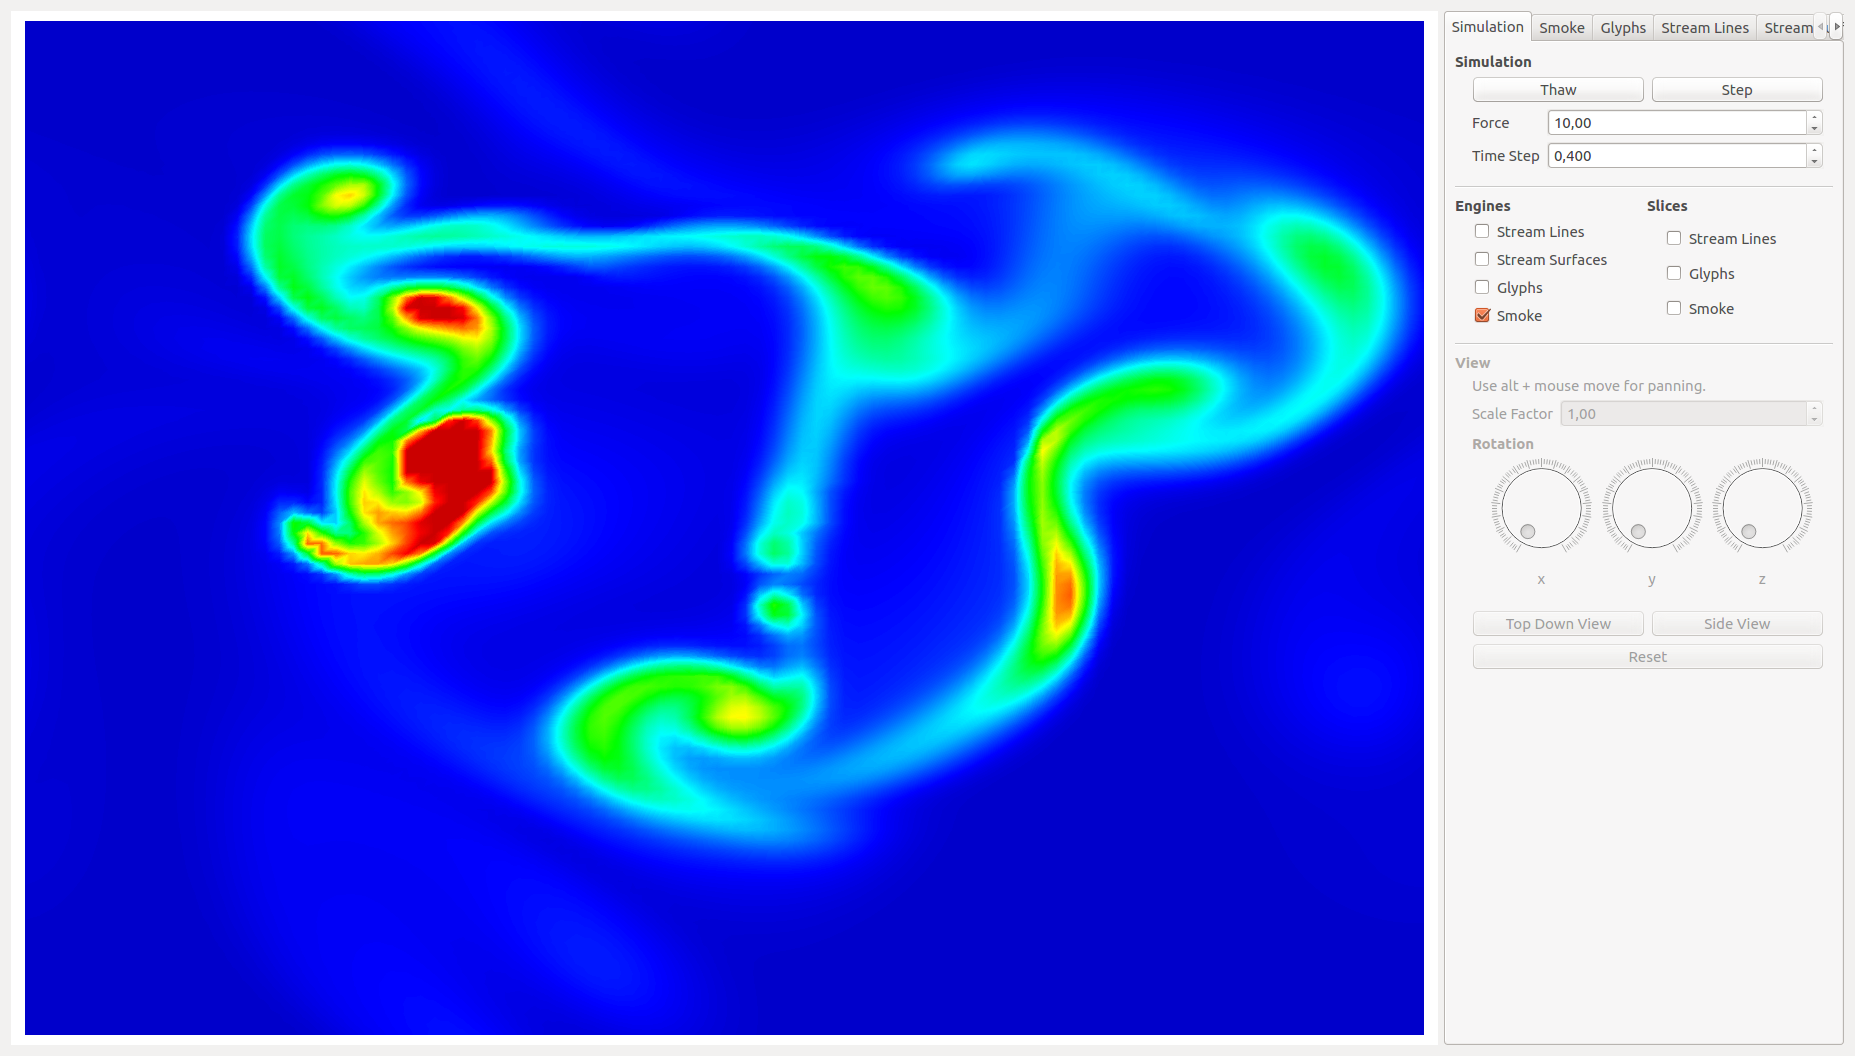
\includegraphics[width=\textwidth, trim={35px 30px 430px 30px}, clip]{colormapping/img/rainbow.png}
		\caption{Rainbow colormap, using $\VarDX = 0.8$.}
		\label{fig:colormapping:intro:differntColorMaps:rainbow}
	\end{subfigure}
	\begin{subfigure}{0.44\textwidth}
		\centering
		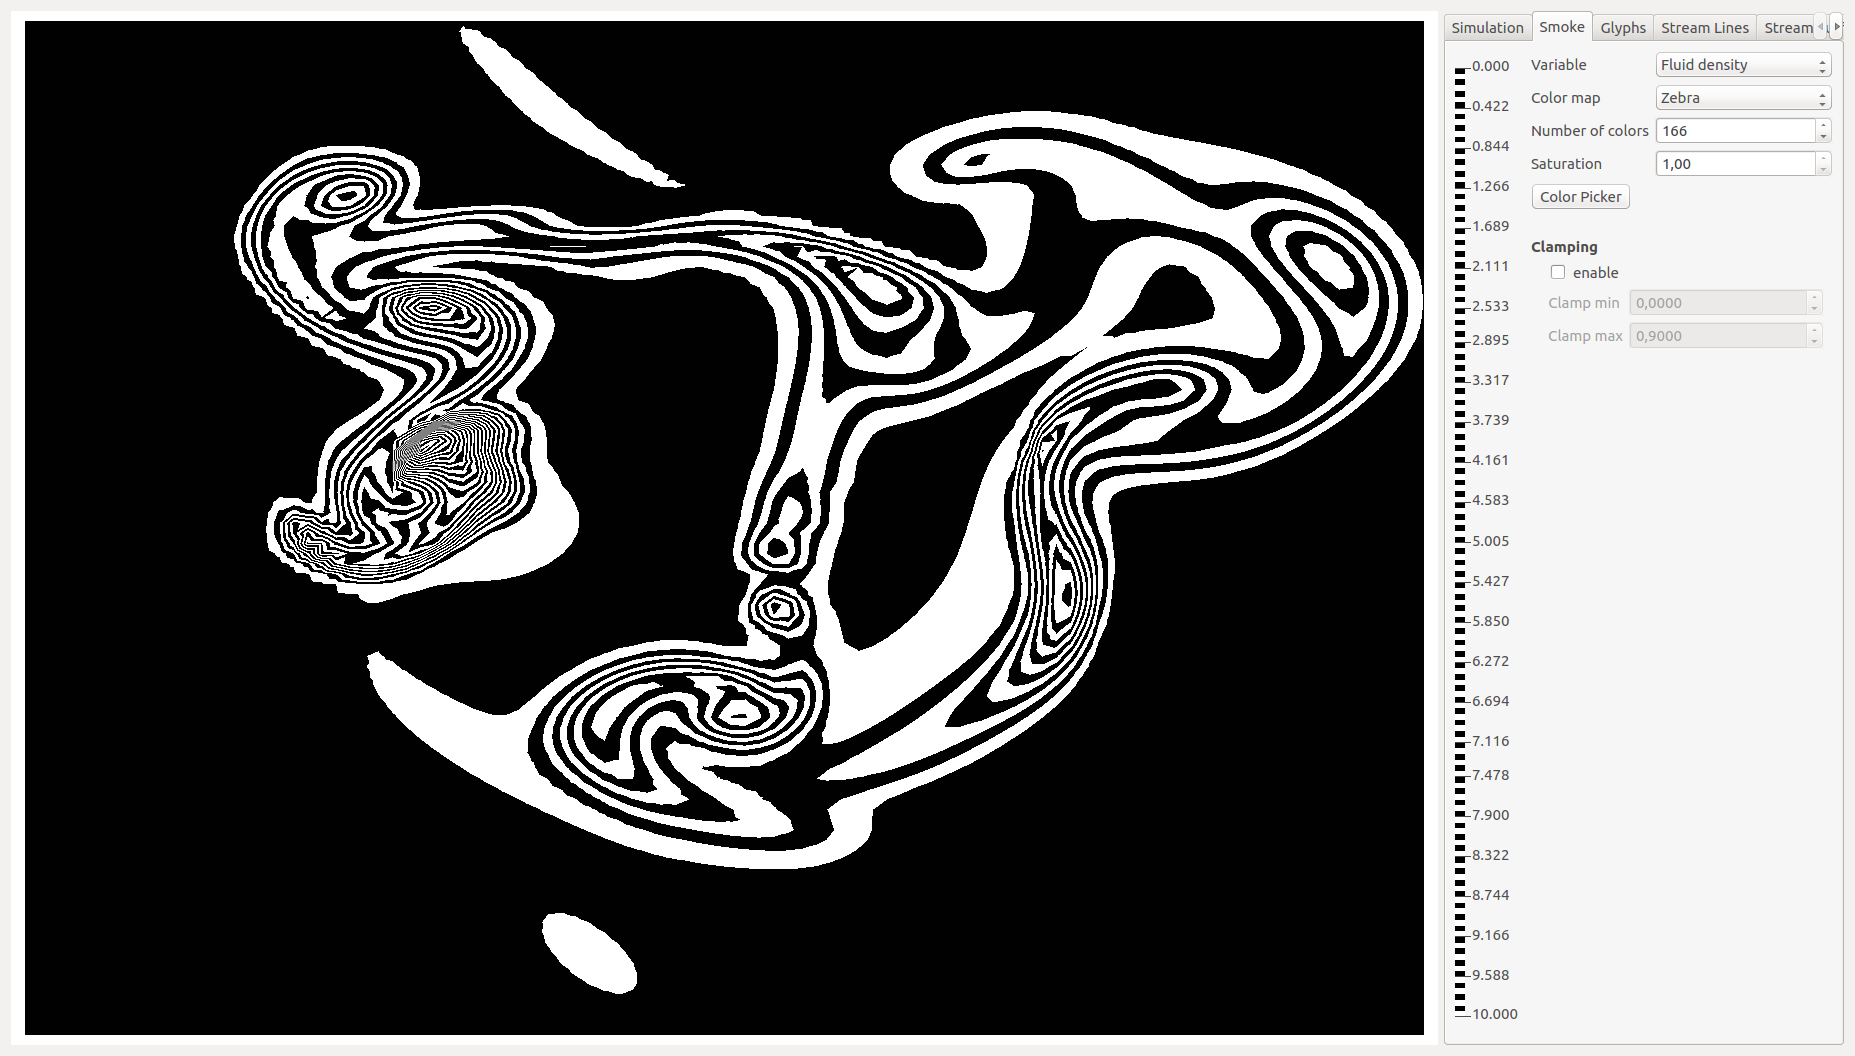
\includegraphics[width=\textwidth, trim={35px 30px 430px 30px}, clip]{colormapping/img/zebra}
		\caption{Zebra colormap showing the first derivative.}
		\label{fig:colormapping:intro:differntColorMaps:zebra}
	\end{subfigure}	
	\begin{subfigure}{0.44\textwidth}
		\centering
		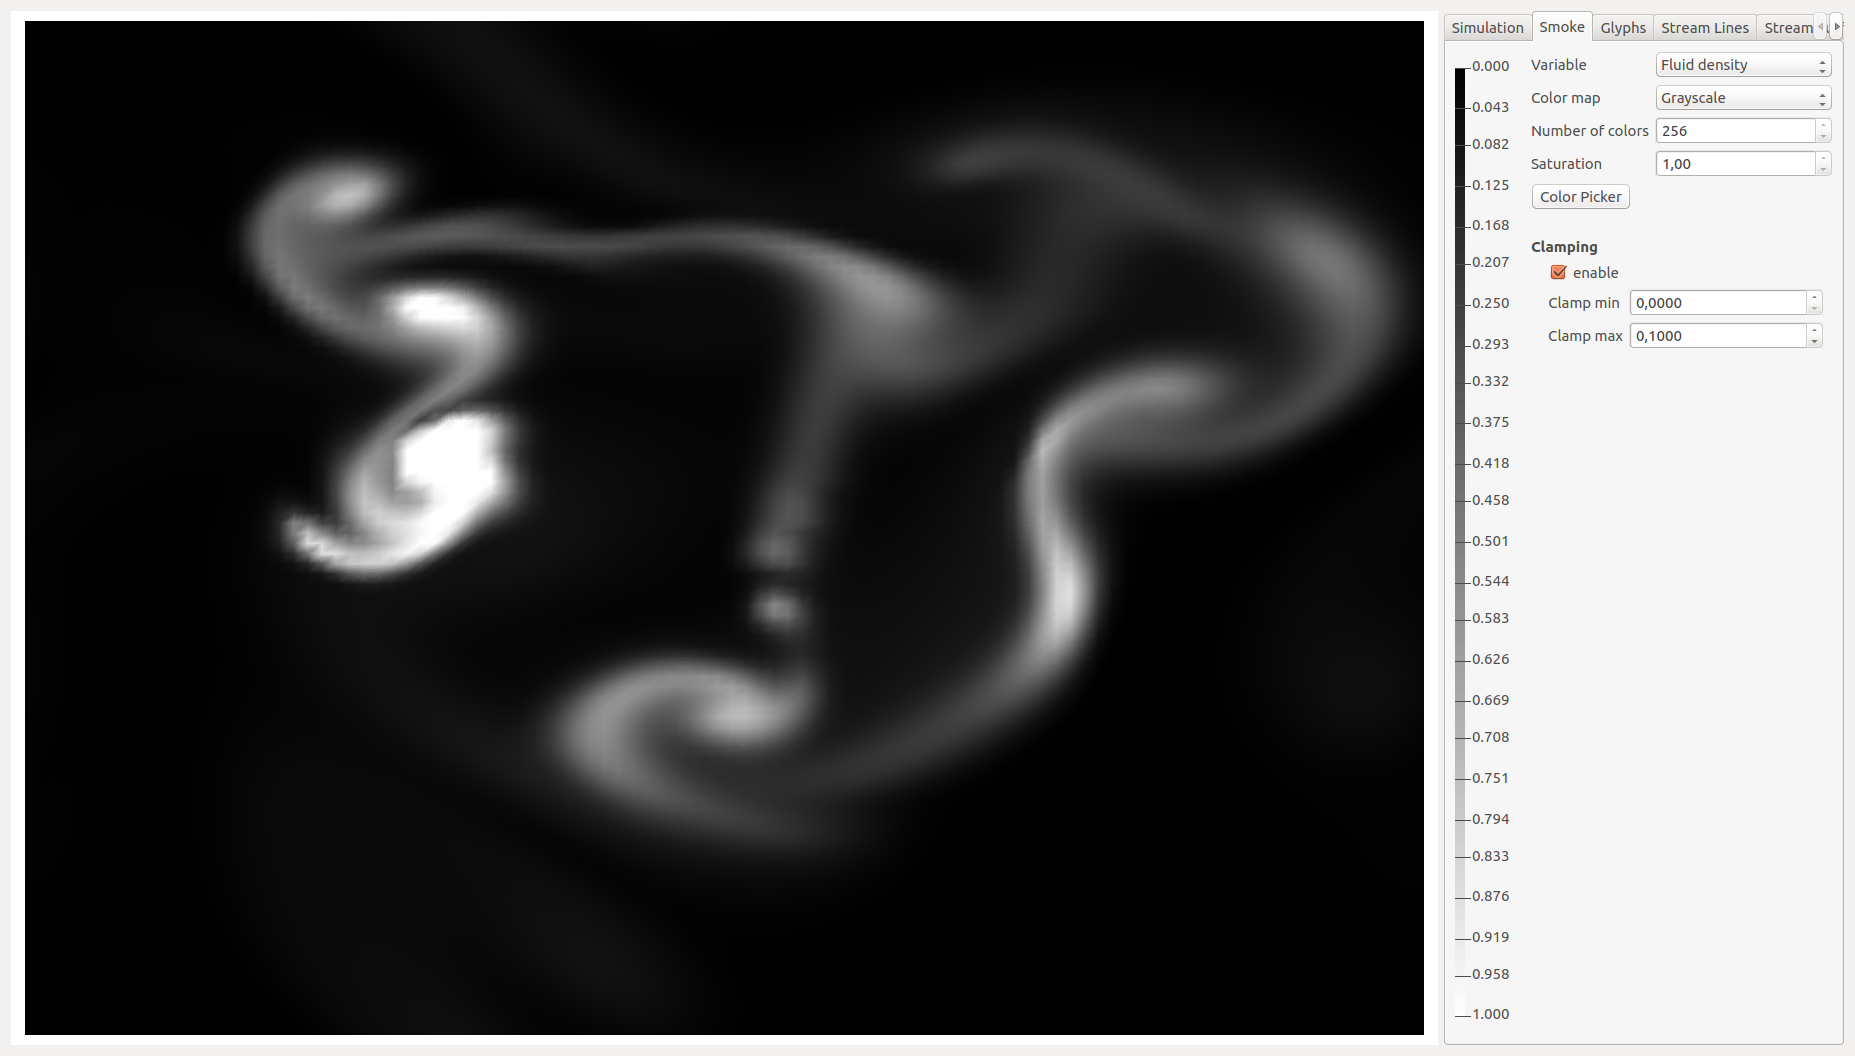
\includegraphics[width=\textwidth, trim={35px 30px 430px 30px}, clip]{colormapping/img/grayscale}
		\caption{Gray-scale colormap.}
		\label{fig:colormapping:intro:differntColorMaps:grayscale}
	\end{subfigure}	
	\begin{subfigure}{0.44\textwidth}
		\centering
		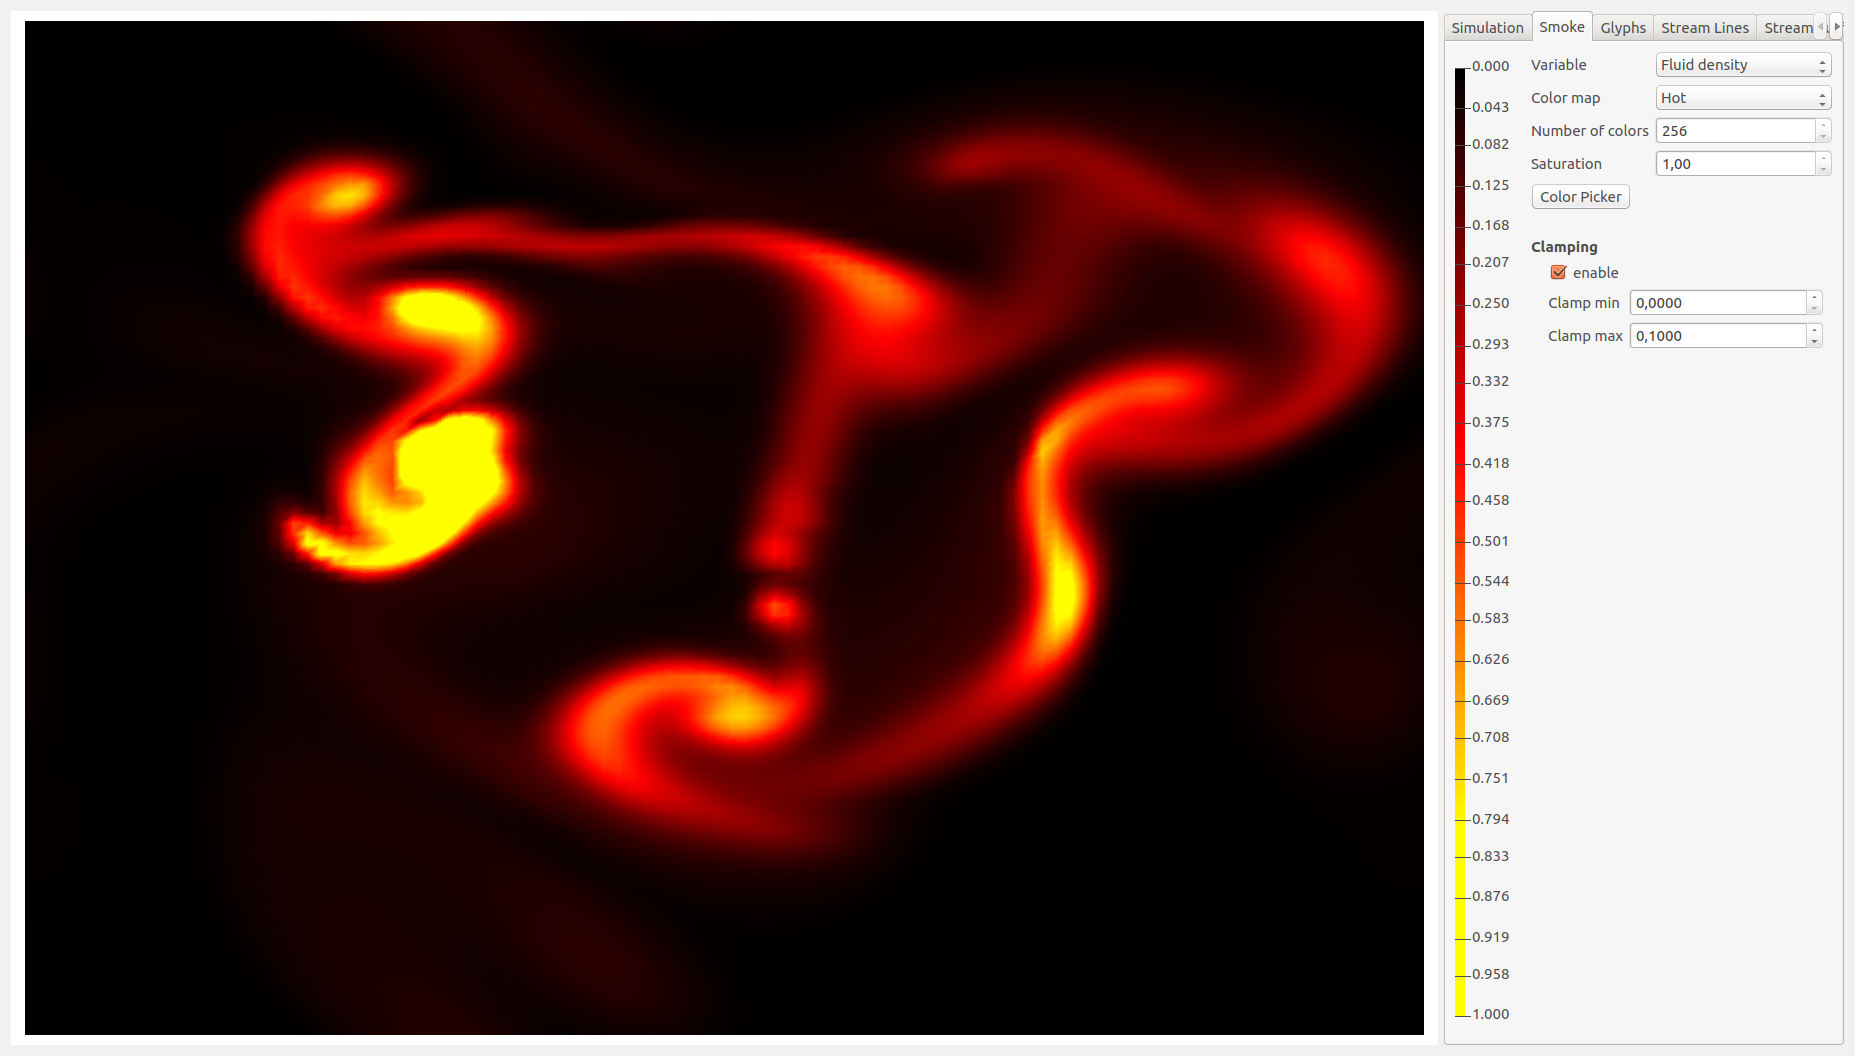
\includegraphics[width=\textwidth, trim={35px 30px 430px 30px}, clip]{colormapping/img/heat.png}
		\caption{Heat colormap.}
		\label{fig:colormapping:intro:differntColorMaps:heat}
	\end{subfigure}
	\begin{subfigure}{0.44\textwidth}
		\centering
		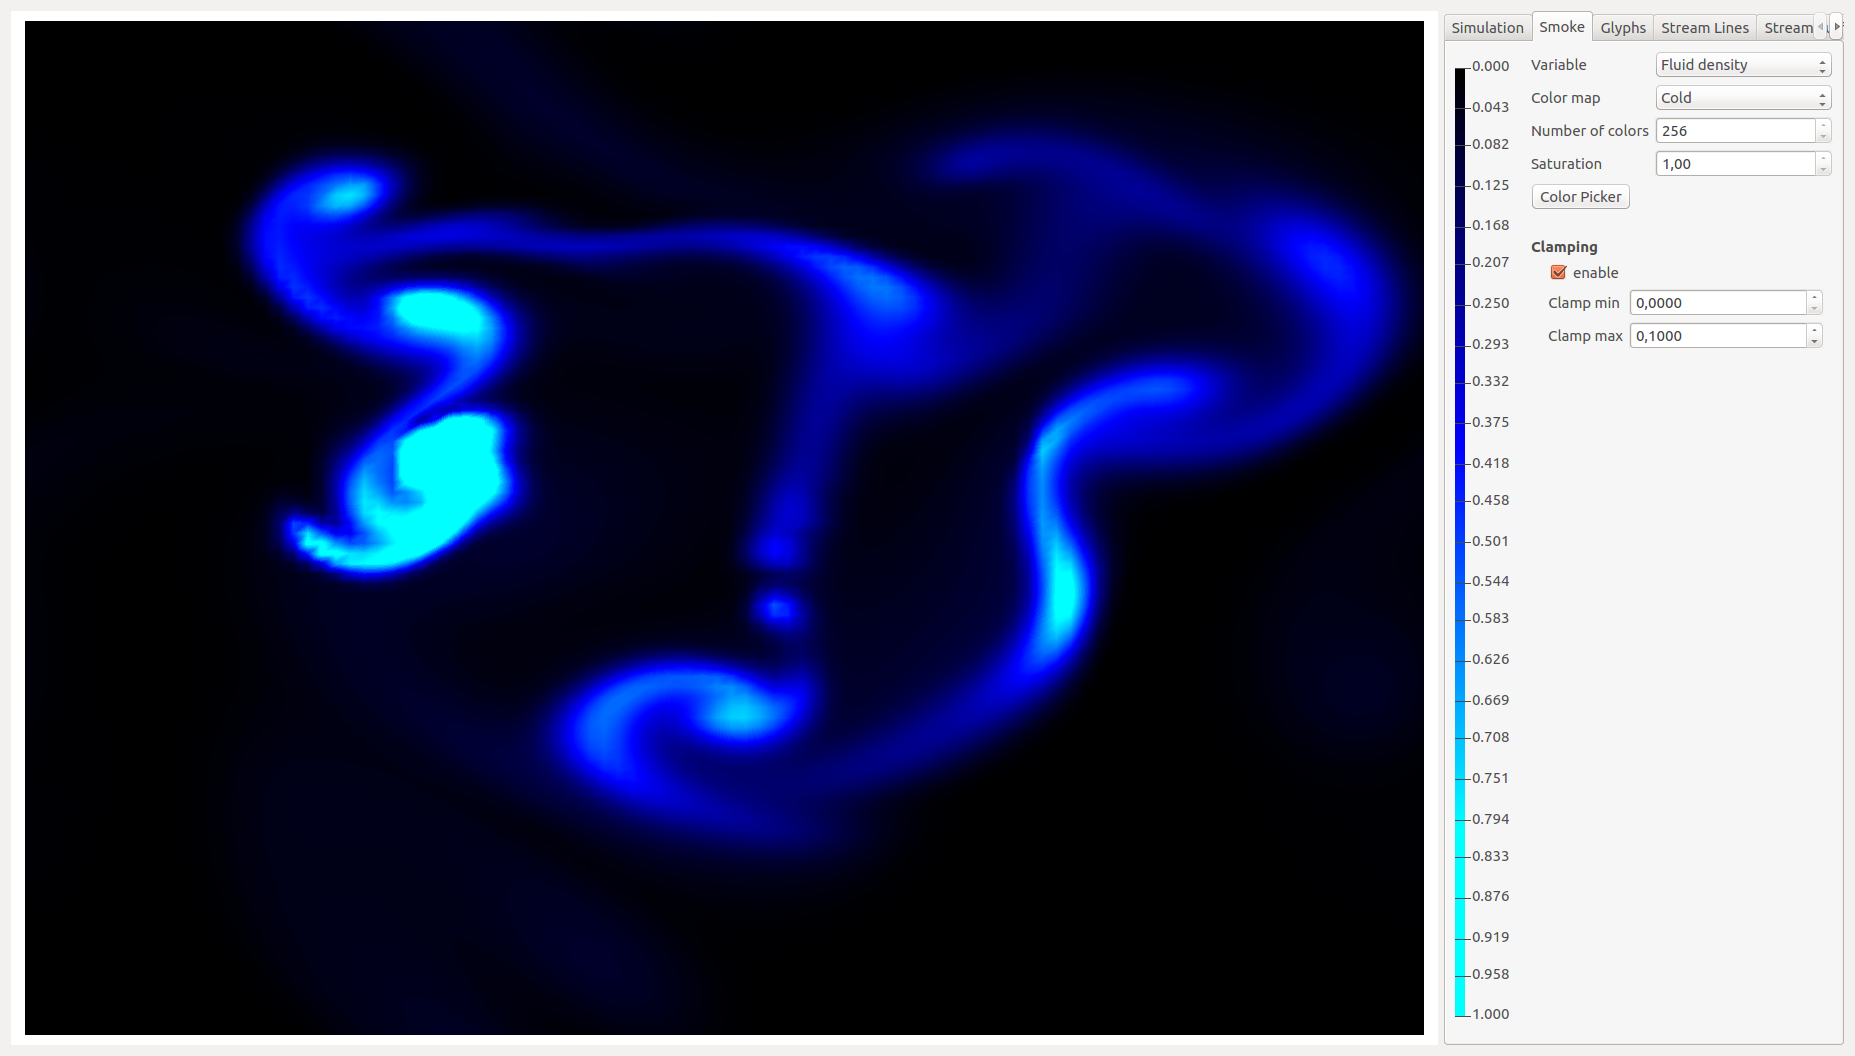
\includegraphics[width=\textwidth, trim={35px 30px 430px 30px}, clip]{colormapping/img/cold.png}
		\caption{Cold colormap.}
		\label{fig:colormapping:intro:differntColorMaps:cold}
	\end{subfigure}
		\begin{subfigure}{0.44\textwidth}
		\centering
		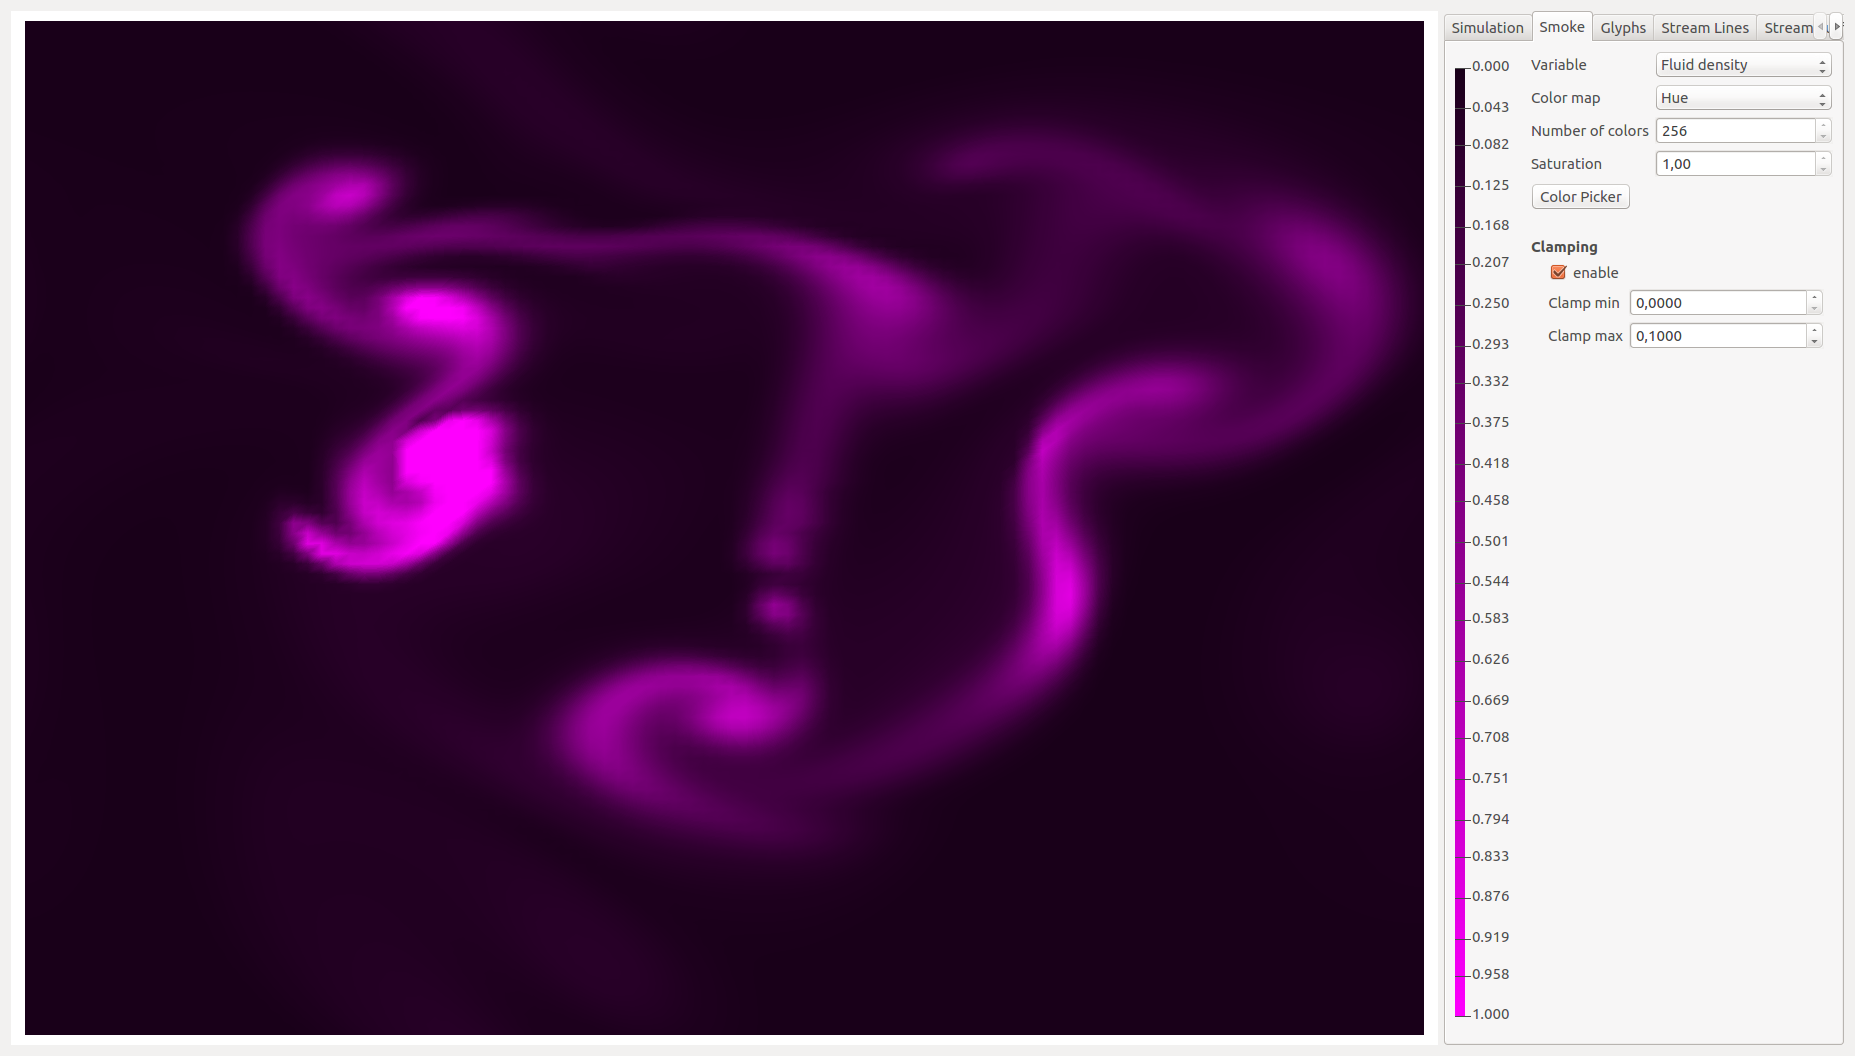
\includegraphics[width=\textwidth, trim={35px 30px 430px 30px}, clip]{colormapping/img/hue.png}
		\caption{Hue colormap using pink hue selected by user.}
		\label{fig:colormapping:intro:differntColorMaps:hue}
	\end{subfigure}
	\begin{subfigure}{0.44\textwidth}
		\centering
		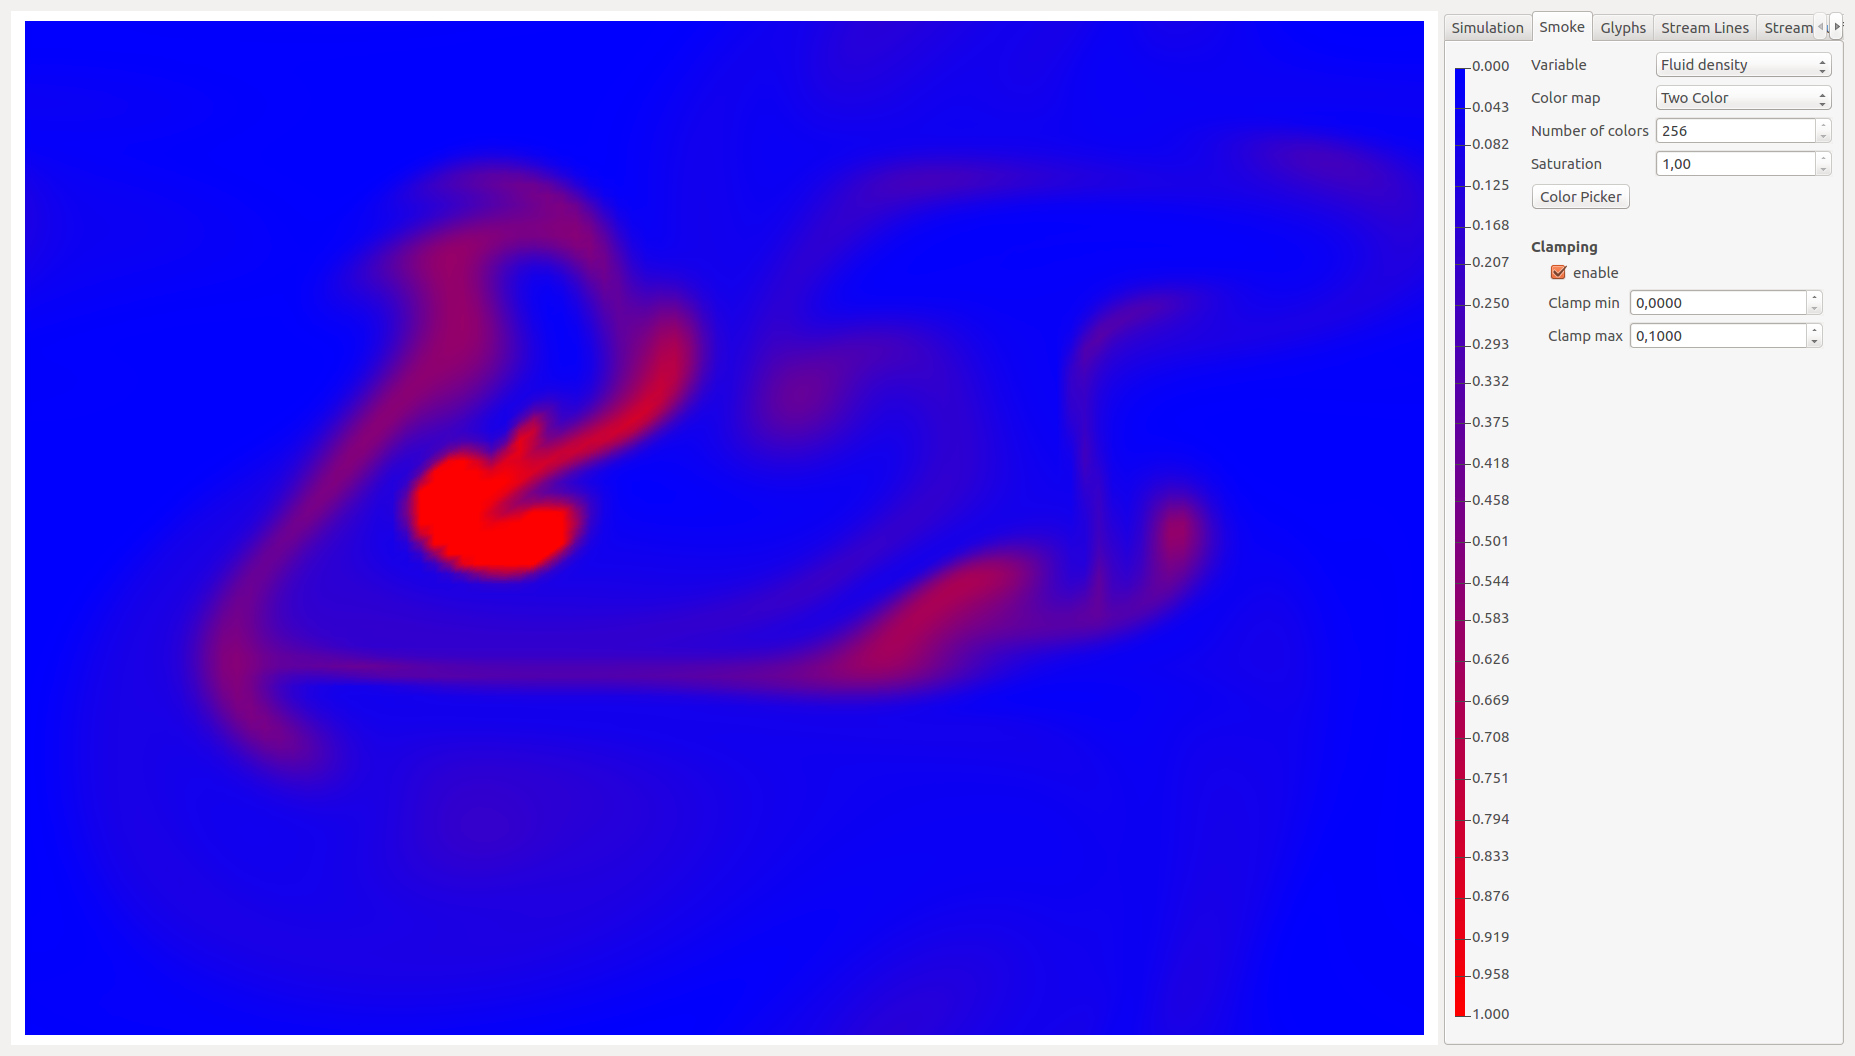
\includegraphics[width=\textwidth, trim={35px 30px 430px 30px}, clip]{colormapping/img/twocolor}
		\caption{Two-color colormap.}
		\label{fig:colormapping:intro:differntColorMaps:twocolor}
	\end{subfigure}	\begin{subfigure}{0.44\textwidth}
		\centering
		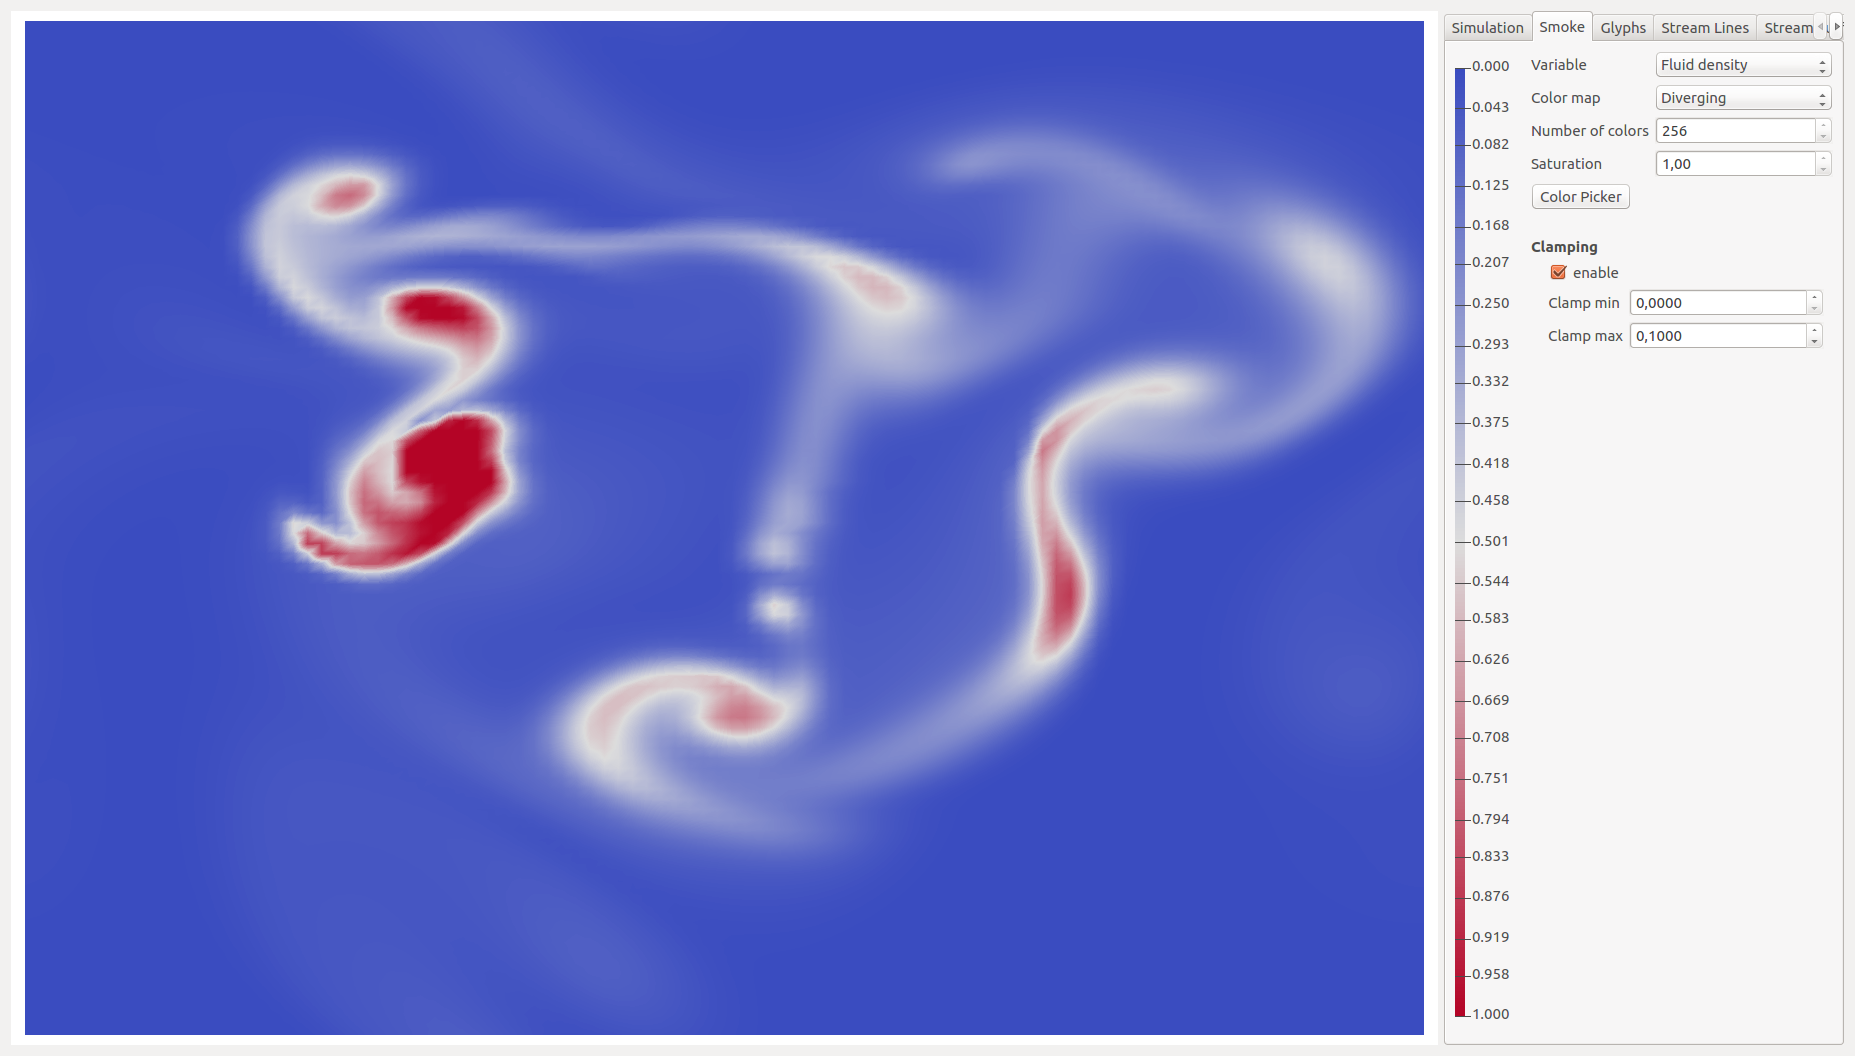
\includegraphics[width=\textwidth, trim={35px 30px 430px 30px}, clip]{colormapping/img/diverging}
		\caption{Blue red diverging colormap.}
		\label{fig:colormapping:intro:differntColorMaps:diverging}
	\end{subfigure}				

	\caption{A visualization of the \emph{Fluid Density} using different colormaps available in the application. All colormaps the full range of availab}
	\label{fig:colormapping:colormaps}
\end{figure}


\subsection{Rainbow colormap} % (fold)
\label{ssub:rainbow_colormap}
The rainbow colormap is, despite its flaws, one of the most used colormaps in the scientific community. The colormap is often seen as visual appealing and gives an intuitively mapping of high and low values to warm (red) and cold (blue) colors. However, when the scalar value does not represent a temperature this mapping might be less intuitive which makes the colormap harder to use.

\subsubsection{Flaws} % (fold)
\label{ssub:flaws}
The rainbow colormap is not only often used, but also often critiqued\cite{borland2007rainbow}\cite{divergingMoreland2009}. Besides the sometimes unintuitive associated of high and low values with warm and cold colors the colormap has some more (serious) flaws. 


% subsubsection flaws (end)



\subsection{Gray Scale colormap} % (fold)
\label{ssub:gray_scale_colormap}
	% GrayScale ColorMap
	\todo[inline]{Discuss GrayScale color map: advantages, disadvantages}

Disadvantages: surface shading, same luminance may look different depending on the surrounding pixels.
% subsubsection gray_scale_colormap (end)
	% ColorMap of Choice
	\todo[inline]{Discuss Chosen color map: advantages, disadvantages, why this one}

\subsection{Heat, Cold, and Hue Colormap} % (fold)
\label{sub:heat_and_cold_colormap}

% subsection heat_and_cold_colormap (end)
\subsection{Diverging Colormap} % (fold)
\label{sub:diverging_colormap}

% subsection diverging_colormap (end)

\subsection{Zebra Colormap} % (fold)
\label{sub:zebra_colormap}

% subsection zebra_colormap (end)
% section color_maps (end)